\chapter{Lösungsentwicklung}
\label{cha:Lösungsentwicklung}
Um eine Lösung zu dieser 

\section{Arbeitsmethodik}
Da in diesem Projekt eine konkrete Aufgabenstellung selbst zu erarbeiten war, und keine konkreten, lieferbaren Objekte vorgesehen waren, wurde zu Beginn eine explorative ad-hoc Methodik verfolgt. Dabei wurde im Projektteam wöchentlich der bisherige Fortschritt analysiert und weitergehende Schritte besprochen. So wurde gewährleistet, dass in der Anfangsphase eine geeignete Aufgabenstellung gefunden werden kann.
\par
Sobald die Aufgabenstellung gefunden wurde, wurde in ein iterativ- inkrementelles Modell gewechselt. Die wöchentlichen Besprechungen wurden beibehalten, um den Fortschritt des Produkts zu verfolgen.

\section{Systemübersicht IoT}
\label{sec:Setup_IoT}
Übersicht: Raspis, Schliessfächer etc...
\begin{figure}
\centering
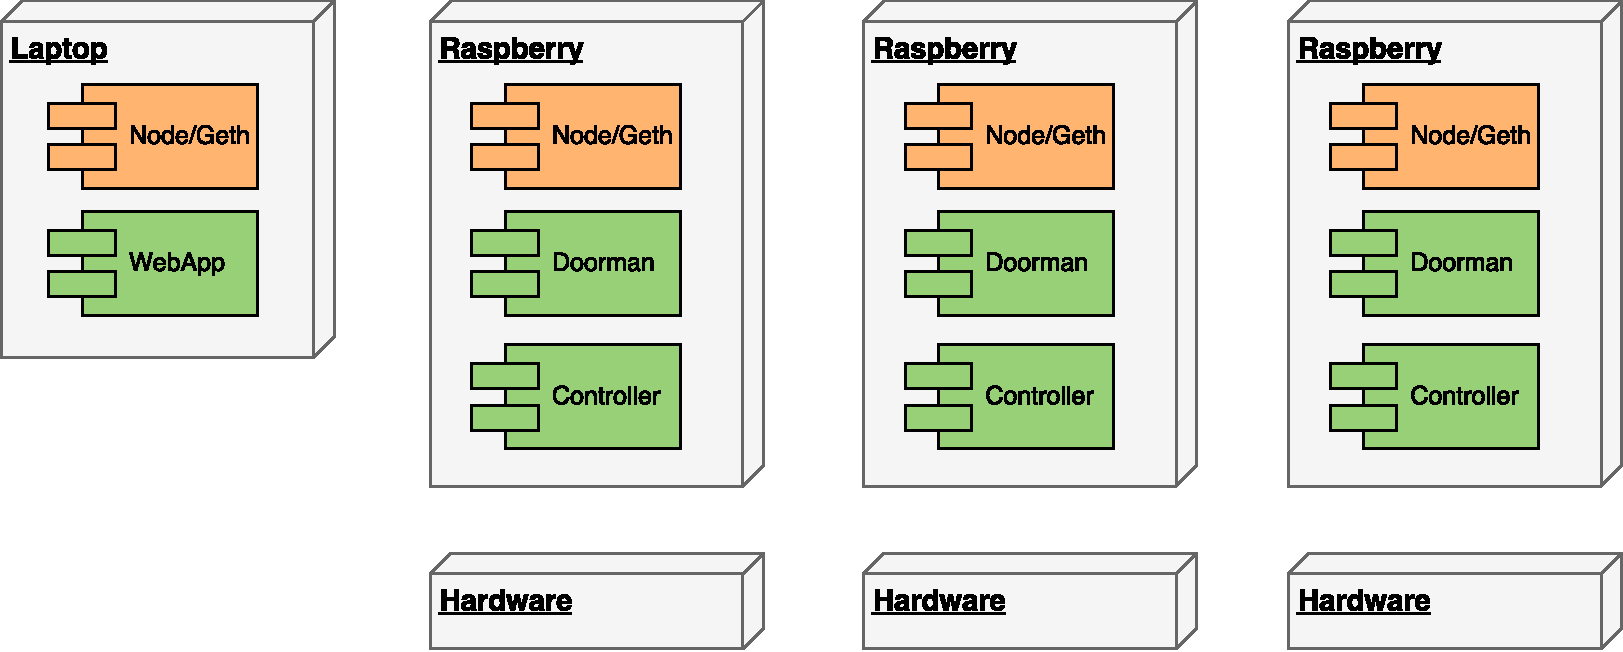
\includegraphics[width=.95\textwidth]{Aufbau_Komponenten} %{CS0031}
\caption{Komponenten und Schnittstellen}
\label{fig:Komponenten und Schnittstellen}
\end{figure}
\subsection{Systemkontext}

\subsection{Systemkomponenten}

\begin{figure}
\centering
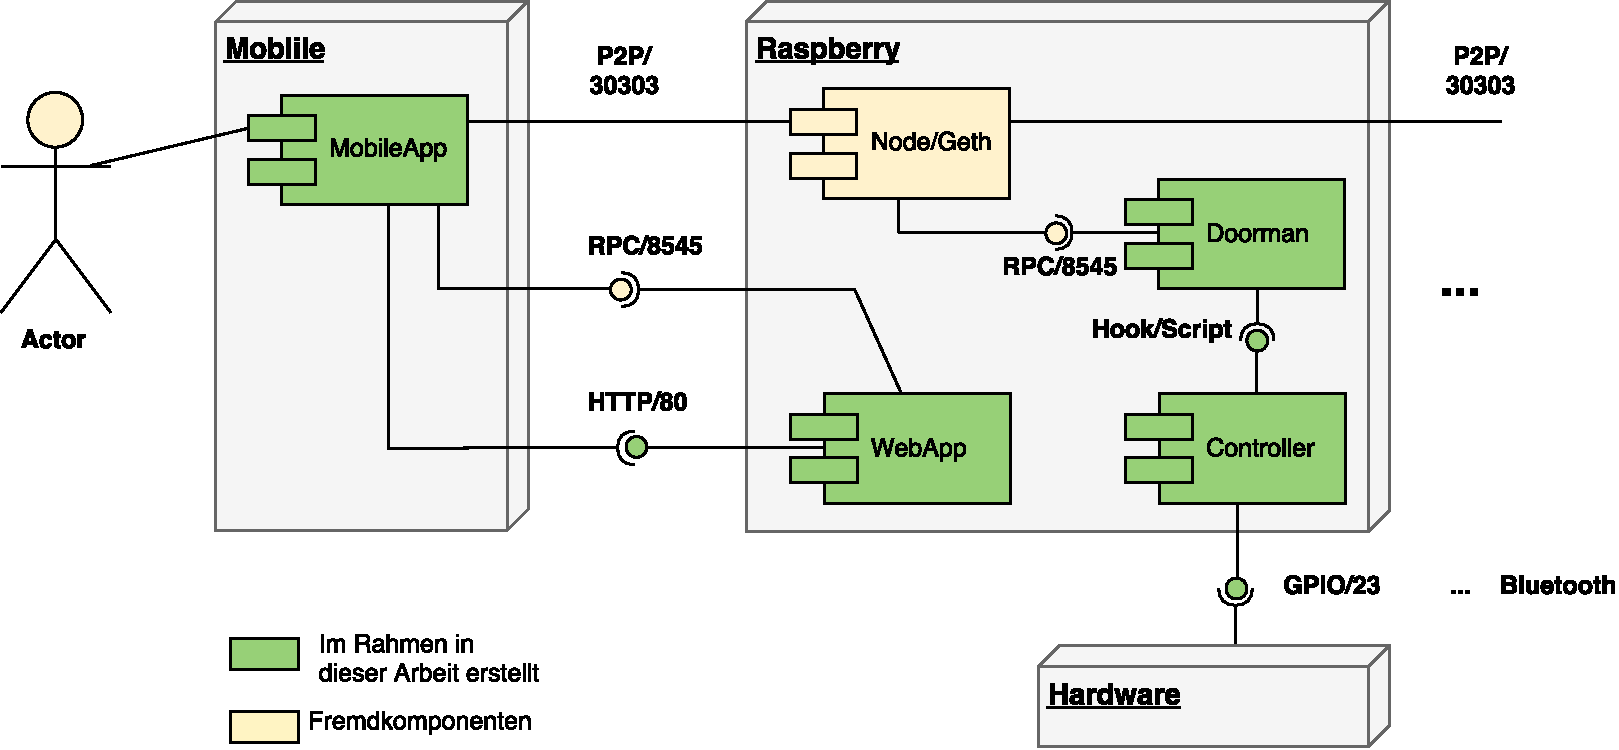
\includegraphics[width=.95\textwidth]{Aufbau_Komponenten_Interface} %{CS0031}
\caption{Komponenten und Schnittstellen}
\label{fig:Komponenten und Schnittstellen}
\end{figure}



\section{Blockchain}
\label{sec:Blockchain}
referenz, verweise

\subsection{Verwendete Implementation}
Wieso Ethereum?

\subsubsection{Ethereum}
\paragraph{Ledger?}
\paragraph{Solidity}
\paragraph{Whisper}
\subsubsection{IBM Hyperledger}
\paragraph{Fabric}
\paragraph{Chaintool}

\subsection{Testchain}

\subsection{Private chain mit Ethereum}


\subsection{Smart Contracts}
\label{subsec:Smart_Contracts}
\epigraph{''A computerized transaction protocol that executes the terms of a contract.``} \cite{BlockchainRevolution}
\\Mit diesem Zitat kann grob das Ziel von Smart Contracts beschrieben werden. Verträge, die in einem maschinenlesbaren Format verfasst sind, können mit unmissverständlicher Präzision und ohne Interpretationsspielraum definiert werden. So ist es möglich, einen deterministischen, digitalen Vertrag zu verfassen.
Entgegengesetzt ist es nahezu unmöglich eine Menge von Smart Contracts angesichts einer unüblichen Situation deterministisch abzuarbeiten. -> http://www.ibtimes.co.uk/pwc-blockchain-expert-pinpoints-sources-ambiguity-smart-contracts-1575778

\susubsection{Erstellen}
Um einen Smart Contract zu erstellen, wird mittels einer geeigneten Programmiersprache dieser formell definiert. Dieser geschriebene Programmcode kann mittels einer Transaktion in die Blockchain eingesetzt werden, wobei Initialwerte angegeben werden. Man sprich hierbei vom erstellen einer Instanz des Smart Contracts, ähnlich wie in der objektorientierten Programmierung. Bei der ausgelösten Transaktion gilt es zu beachten, dass diese keinen Empfänger hat; der Empfänger dieser Nachricht ist die Blockchain selbst. Wie bei jeder Transaktion eine gewisse Menge gas mitgegeben werden, damit die Operation abgeschlossen werden kann. Wenn der Code in die Blockchain eingesetzt wurde, erhält diese Instanz des Contracts eine Adresse, über die später mit dieser spezifischen Instanz interagiert werden kann.
Beim Erstellen eines Smart Contracts wird auch ein abi generiert. Dieses beschreibt die möglichen verfügbaren Attribute des Contracts und die Interaktionsmöglichkeiten (\#VGL. Funktionen) inklusive deren allfällige Parameter und Rückgabewerte (\#VGL. Interfacedeklaration in OO Sprachen).

\susubsection{Lesezugriff}
Um ein Attribut auszulesen oder eine Funktion mit konstantem Rückgabewert auszuführen, kann diese über ein verfügbares Interface, wie die JavaScript console von geth, direkt aufgerufen werden. Bei Funktionen mit konstantem Rückgabewert ist zu beachten, dass diese nur auf der lokalen Node emuliert werden (CITATION NEEDED) und es somit nicht möglich ist, eine Änderung in der Blockchain zu bewirken. Diese Funktionen haben folglich nur Lesezugriff.

\subsubsection{Schreibzugriff}
Wenn eine Funktion auf der Instanz aufgerufen wird, die eine Änderung in der Blockchain bewirkt, muss eine Transaktion ausgelöst werden. Der Sender der Transaktion muss dabei für die Kosten für gas und allfällige weitere Kosten (\#VGL. Bezahlbare Funktionen) aufkommen. Der Sender kann nicht nur ein Account sein, sondern auch ein weiterer Smart Contract, an dessen Adresse genügend Ether liegt, um die Transaktionskosten zu begleichen.

\paragraph{Bezahlbare Funktionen}
Einige Funktionen benötigen mehr Ether als nur die gas-Kosten. Wenn beispielsweise eine Dienstleistung oder Sache über einen Smart Contract verkauft werden soll, muss noch eine Menge Ether als Zahlungsmittel überweisen werden. Die Menge Ether ist im Smart Contract festgelegt und kann durch Inspektion des Programmcodes eingesehen werden. Sollte der Kunde zu wenig Ether schicken, kann der Smart Contract definieren, dass die Transaktion nicht erfolgreich ist und der Kunde sein Geld zurückerhält. Dazu kann die Transaktion selbst als nichtig erklärt werden und es muss nicht auf das Withdrawal Muster zuückgegriffen werden.

\subsubsection{Solidity}
Solidity ist eine Programmiersprache zur Erstellung von Smart Contracts auf der \acrfull{EVM}, die syntaktisch stark an JavaScript angelehnt ist. Sie kann auch auf anderen Blockchain Platoformen (wie Tendermint oder Counterparty für Bitcoin) verwendet werden. -> https://www.cryptocoinsnews.com/counterparty-brings-ethereum-smart-contracts-to-the-bitcoin-blockchain/\\Solidity wird, in Anlehnung auf den Ausdruck object-oriented, als contract-oriented beschrieben, da die erstellenden Konstrukte in der Sprache als ''contract`` und nicht ''object`` bezeichnet werden. Inhaltlich beziehen sich die beiden Ausdrücke auf dasselbe Konzept.

\subsubsection{Gängige Muster - GEHÖRT DAS INS KAPITEL "SMART CONTRACTS" ODER HIERHIN?}
Folgend werden einige Muster aufgelistet, die beim Entwurf und der Implementation von Smart Contracts mit Solidity, aufgrund der inhärenten Architektur der Platform und Sprache, beachtet werden sollten. Diese Muster dienen als Richtlinie und umgehen bekannte Limitationen oder schliessen Sicherheitslücken. Es ist möglich unter Misachtung der Muster Smart Contracts zu entwickeln. -> \#ALLE BEISPIELE VON http://solidity.readthedocs.io/en/develop/
\#Alle folgenden Beispiele waren für die Erarbeitung der Rentable \& RentableDiscovery Contracts zu beachten!

\paragraph{Generell}
Instanzen von Smart Contracts erhalten, wie Accounts, ebenfalls eine Adresse, an die Ether geschickt werden kann. Meistens wird dies in Form von Funktionsaufrufen gemacht, allerdings kann auch direkt an einen Smart Contract Ether überwiesen werden. Hierbei ist es wichtig zu beachten, dass der Ether zurückerstattet wird, der aus Veresehen an diesen gesendet wurde (\#VGL Withdrawal Muster).

\paragraph{Withdrawal Muster}
Wenn aus einem Smart Contract eine Transaktion an eine Adresse gestartet wird, muss das gas dafür vom digitalen Vertrag bezahlt werden (oder besser: vom Account, der die ursprüngliche Transaktion an den ersten digitalen Vertrag gestartet hat). Im Fall einer einfachen Überweisung fallen keine gas-Kosten an. Ist das Ziel aber ein anderer Smart Contract, besteht die Möglichkeit, dass der Zielvertrag Code ausführt, wenn er eine Transaktion erhält. Das Withdrawal Muster wird folglich verwendet, um zu verhindern, dass der Quellvertrag dies überprüfen muss oder für die gas-Kosten des anderen Smart contracts aufkommen muss.

Wird das Withdrawal Muster angewendet, überweist ein Smart Contract Ether nicht direkt an eine Zieladresse. Stattdessen merkt er sich die Menge, die einer Zieladresse zusteht und stellt die Möglichkeit zur Verfügung, dass diese Begünstigten Ether abheben können. Dies findet mittels einer Transaction statt, die vom Begünstigten ausgelöst werden muss. Die gas-Kosten für diese Art Funktionen sind meist vernachlässigbar und werden durch die zurückerhaltene Menge Ether kompensiert. Da der Begünstigte die Adresse des Quellvertrags kennt und den Quellcode von Smart Contracts öffentlich ist, kann die Zieladresse sicher gehen, beim aufrufen dieser withdrawal-Funktion auf dem Quellvertrag auch tatsächlich die Menge Ether zurückzuerhalten.
http://solidity.readthedocs.io/en/develop/common-patterns.html\#withdrawal-from-contracts

\#möglicherweise ein bildli zeichnen oder beispielcode einfügen


\paragraph{Re-Entrancy}
Hierbei handelt es sich um ein Muster, das angewendet wird, wenn in einem Smart Contract A ein interner Zustand existiert, der die Menge an Ether speichert, der \emph{anderen} zusteht und eine Möglichkeit besteht, diese Menge Ether zu entnehmen (\#VGL. Withdrawal Muster). Beispiele für zurückzuerstattenden Ether kann ein Gebot in einer Auktion sein oder Depots wie bei lokkit.
Unter der Annahme, dass die Zieladresse für die Rückerstattung ein Smart Contract B ist, kann B A angreifen. Bei einer Transaktion wird immer der zugehörige Code ausgeführt. Das heisst, dass B auf eine eingehende Transaktion reagieren kann und ihrerseits erneut die Transaktionsfunktion von A aktivieren kann (\#VGL. Withdrawal Muster). Wenn der Zustand von A noch nicht geändert wurde, wird der Betrag erneut gesendet, bis A kein Ether mehr zur Verfügung hat.

Um mehrfaches Überweisen von Ether zu verhindern, ist es essentiell, zuerst den internen Status des Vertrags zu ändern, bevor Ether überwiesen wird. Die \emph{total} zur Verfügung stehende Menge Ether eines Smart Contracts wird in der Blockchain gehalten und ist Teil des Konsensus. Es ist somit nicht möglich, dass mehr Ether ausgegeben wird als in dem jeweiligen digitalen Vertrag vorhanden ist. 

CODE SNIPPET FALSCH:
    function withdraw() {
        if (msg.sender.send(deposit[msg.sender])) { // das kann mehrere male ausgeführt werden.
            deposit[msg.sender] = 0;
        }
    }
CODE SNIPPET RICHTIG:
    function withdraw() {
        var currentRefund = deposit[msg.sender]; // zurückerstattend Menge auslesen
        deposit[msg.sender] = 0; // momentanes Depot zurücksetzen, bevor überwiesen wird! Dies wehrt die Re-Entrancy Attacke ab
        msg.sender.transfer(currentRefund); // hier transfer anstatt send benutzen, da (\#TODO)
    }

http://solidity.readthedocs.io/en/develop/security-considerations.html\#re-entrancy

\section{Komponenten}
\label{sec:Komponenten}
Nachfolgend werden die einzelnen Komponenten beschrieben, die für die volle Funktionalität der lokkit-Philosophie benötigt werden.
\subsection{Doorman}
Doorman implementiert die IoT-Seite der Benachrichtigungen mitterls Whisper Protokoll.
\subsubsection{Wieso Python? Wieso Python 2.7?}
\subsubsection{Mechanismus}

\subsection{Smart Contracts (Business Logik)}
Die Smart Contracts, die mit Solidity implementiert wurden, werden nachfolgend erläutert. Diese Smart Contracts bilden das Rückgrat der Applikation und bilden die Business Logik in Code Form ab und legen sich als Zugriffslayer zwischen die Userinteraktion und die Blockchain als Datenbank.

\#WICHTIG!!
Erwähnen der shortcomings, da unsere Contracts eine nicht vordefinierte Anzahl Iterationen haben. Dies kann aufgrund des Block-Gas limits zu stalling führen. Auch lese-Operationen, die aus anderen Smart-Contracts aufgerufen werden können diesen zum stallen bringen. -> http://solidity.readthedocs.io/en/develop/security-considerations.html\#gas-limit-and-loops

\subsubsection{Rentable}
\subsubsection{RentableDiscovery}

\subsubsection{Weitere Überlegungen}
noch einen separaten "data-store" für die Reservationen. Nicht-beachtete Konzepte. Raum für Verbesserungen.


\subsection{Frontend}
\subsubsection{Mobile App (Android)}
\paragraph{geth / offizielle API}
\paragraph{Status.io}
mit Verweis auf Testchain

\subsubsection{DApp}
\paragraph{Embark}
\paragraph{Vue.js}

\subsubsection{Command Line Client (geth attach)}


\section{}